% !TEX root = main.tex
\section{Motivation}\label{sec:example}

Model Predictive Control (MPC) refers to the class of control strategies that design control actions by solving a finite horizon optimal control problem at each sampling instant. While each optimization gives a sequence of optimal control actions, only the first action is applied to the process. The same procedure is applied in the next time instance after receiving the updated value of the process state. MPC has shown to be successful in industrial applications since it is able to handle large number of states and control actions and automatically considers constraints in the optimization.

The optimization of each time instance uses a dynamic model of the process to predict the future states and find the optimal sequence of actions that satisfies all the constraints. The objective function of the optimization is usually linear or quadratic. The resulting optimization problem can be cast as a linear program (LP) or quadratic program (QP), respectively, if the dynamic model is linear. For hybrid models with linear dynamics in each mode, the optimization problem can be cast as a mixed integer linear or quadratic program (MILP/MIQP). 

 The main difference between MPC and conventional control is in the nature of the function that maps the measured outputs to control actions. The former computes such a function online but the latter pre-computes it off-line. The required online computations in MPC limits its applicability to slow processes: the sampling time should be large enough to allow enough time for solving the optimization and obtaining the optimal action for the next time instance. Moreover, the optimization solver needs to be certified for using MPC in safety critical applications.
 % while the  therefore that in the latter the control function is pre-computed off-line.
These issues can be tackled using \emph{Explicit MPC} under proper assumptions on the model, constraints and the objective function. Explicit MPC solves the optimization problem off-line over a bounded domain of the state variables by using multiparametric programming techniques. The output of Explicit MPC is the optimal control actions as an ?explicit? function of the states which is piecewise affine. This expands the class of systems being controlled by MPC strategies since the implementation requires only storing a lookup table of linear gains and performing an affine computation using the appropriate gains at each time instance. A survey on Explicit MPC can be found in \cite{Alessio2009}.

\begin{figure}[t]
	\begin{tabular}{cc}
	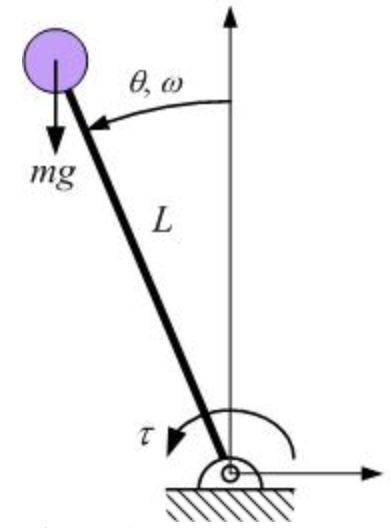
\includegraphics[width=2cm,height=3cm]{Figs/inv_pend.png}&	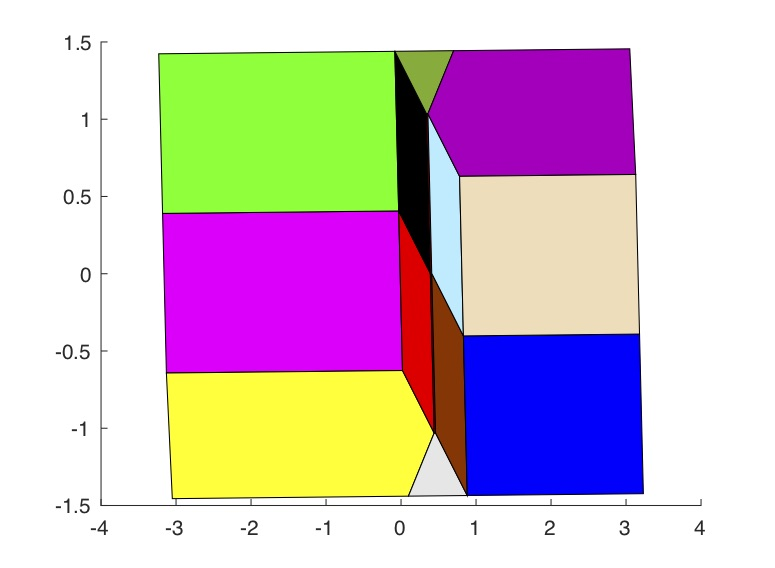
\includegraphics[width=6cm,height=4cm]{Figs/regs.jpg}\\
	(a)&(b)
	\end{tabular}
	\caption{(a) Inverted pendulum; (b) 2-D plot of polyhedral partitions for an explicit MPC applied to the inverted pendulum.}
	\label{fig:inverted_pendulum}
\end{figure}

As an example of a dynamical system, consider the problem of designing a controller for an inverted pendulum depicted in Fig.~\ref{fig:inverted_pendulum}~{(a)}.
The goal of the controller is to keep the pendulum at the vertical position while satisfying hard constraints on the state variables and control inputs.
A model of the system can be constructed using physical principles. After linearization and time discretization, the model is
	\begin{equation}
		\begin{bmatrix}
			 \theta_{k+1}\\
			\omega_{k+1}
		\end{bmatrix}=
		\begin{bmatrix}
			1 & T_s\\
			\frac{T_sg}{L}& (1-\frac{T_sb}{mL^2})		
		\end{bmatrix}
		\begin{bmatrix}
			\theta_k\\
			\omega_k
		\end{bmatrix}+
		\begin{bmatrix}
			0\\
			\frac{T_s}{mL^2}
		\end{bmatrix}u_k + w_k
		\label{eq:pendul_ss}
	\end{equation}
	where $\theta_k$, $\omega_k$ and $u_k$ denote respectively the angular position, angular speed and the input torque at time $kT_s$ with $T_s$ being an appropriate sample time.
	The disturbance $w_k\in\mathbb R^2$ bounded with $\|w_k\|\leq \Delta$ captures the modeling error due to linearization and discretization. The parameter $g=9.81 [m/s^2]$ is the gravitational acceleration, $m$ is the ball mass, $b$ is the rotational fraction coefficient and $L$ is the length of the bar. Starting from an initial state $(\theta_0,\omega_0)$, we would like the system's trajectory to converge to its equilibrium point $\theta=0$ and $\omega=0$, while $\theta_k\in[-\pi,\pi]$ and $\omega_k\in[-\pi/8,\pi/8]$ in all time instances.\\
	There are many control schemes that can guarantee convergence of the trajectories to the rest position (e.g., state feedback or linear quadratic regulator), but fail to ensure hard constraints on the states at all time instances. The main feature of MPC schemes is to automatically include these constraints in the design of control actions.
	%
	%  adding polytopic constraints, MPC schemes will be the best choice. 
	%In literature, many control schemes are proposed for stablizing the system around the equilibrium point. 
	%In order to design a controller which takes additional safety constraints are taken into account, model predictive control (MPC) schemes seem to be best candidate. 
	One major challenge of implementing model predictive controllers over embedded systems is to solve the related optimization within each sampled time inerval. Since the system under consideration is LTI, one can use explicit MPC \cite{Bemporad:2002} that computes partitions over state space together with affine functions which are then used to compute the optimal control input over their corresponding partition. For the inverted-pendulum example, the computed controller contains $12$ partition presented in Fig.~\ref{fig:inverted_pendulum}~{(b)}, each with an affine function that gives the control action over that partition.
	
	%To overcome this issue, in [Bemporad:2002], explicite MPC, a multi-parametric programming based approach is proposed for LTI systems. 
	In many practical applications, explicit MPC is implemented over relatively low-price embedded systems with limited memory capacity and computational power. The partitions together with the affine functions should be stored on the embedded system.
	Computing the control action, i.e., evaluating the affine function for a specific state, can be performed efficiently using for example binary tree search. However, the memory limitations is more crucial since the memory usage increases linearly with the number of partitions.
	In this paper we discuss a method for reducing the memory usage in applying explicit MPC to LTI dynamical systems.
	%The goal of this paper is to propose a mTherefore, we would like to explore ways to reduce the required memory for storing the controller efficiently.
	
	Many low-end embedded systems only support fixed point arithmetic which causes errors that is inversely proportional to the number of bits used for representing each variable. It is necessary to account for such errors in the design stage of the controllers to be able to enforce hard constraints on the states at the final implementation of the controller. Our proposed method iteratively solves a robust version of the MPC with varying bound on the disturbance to include such errors.   %Therefore, one needs to formulate the problem as robust EMPC to count for disturbance input $|\delta|\leq \Delta$ which is summed up with the control input torque $u$ in each time step.
	 %Setting the number of bits for storing different variables, one can compute the upper bound for approximation error, $\bar\omega$.
	%However, we would like to achieve the minimum number of bits to reduce memory requirements.
	
	In summary, we design a robust explicit MPC, taking fixed-point arithmetic errors into account and find a minimal set of mixed precision assignments for all the quantities that must be stored on the embedded system. Denote the overall error produced by the fixed finite precision implementation by $e$.
	%Denote the total number of bits required for implementation of RMPC by $N_b$. Given the maximum memory budget denoted by $\bar N_b$, the overall goal will be to design a robust MPC that (i) achieves the performance objectives including hard constraints and (ii) is implemented in a way that $N_b\leq \bar N_b$.
   The overall goal will be to (i) design a robust MPC that achieves the performance objectives including hard constraints while the error because of the fixed-point implementation is taken into account and (ii) to minimize the total number of bits that are required for storing the computed RMPC over the embedded system while $e\leq \Delta$ is satisfied.
	%while the error resulted by fixed-point arithmetic is smaller than the error bound $\Delta$.
	Our approach iteratively expand the bound on disturbance $\Delta+\Delta_0$, designs a robust explicit MPC controller with this bound and uses state-of-the-art fixed-point error analyzers to find the minimum total number of bits for storing the controller into the embedded system with maximum error $\Delta_0$.\\
	
	Figure \ref{fig:overview} gives a high-level overview of our proposed setup. 
	%We start with defining the memory budget $\bar N_b$ and an initial bound $\Delta_0$. For the inverted pendulum example, we choose $\bar N_b=6000$ and $\Delta_0=0$. 
	We start with defining an initial bound $\Delta_0$. For the inverted pendulum example, we choose $\Delta_0=0$. To design robust explicit MPC, MATLAB is run and the output of the controller is computed. Next, we ask Daisy to provide us with a mixed-precision scheme respecting the error bound $\Delta$. However, $\Delta_0=0$ is not realizable as error resulted from fixed-point implementation is always greater than zero. Therefore, we go ahead and increase $\Delta$ by $0.05$. Solving the robust explicit MPC problem for the new disturbance bound gives the new controller. Next, we ask Daisy to provide us with fixed-point precision for all the parameters such that the new bound is respected. The mixed-precision scheme given by Daisy results in total number of bits $6084$ for the corresponding robust explicit MPC. The mixed precision implementation takes about $10\%$ less memory compare to the smallest uniform precision that respects $\Delta$. 
	%The mixed-precision scheme given by Daisy results in total number of bits $N_b=6084$ and since $N_b>\bar N_b$, we increase $\Delta$ again. Increasing $\Delta$ by $0.1$, Daisy provides us with a mixed-precision scheme with $N_b=5900$ for the corresponding robust explicit MPC. As $N_b<\bar N_b$ the algorithm stops. The mixed precision implementation takes $11\%$ less memory compare to the smallest uniform precision that respects $\Delta$. 
%	Using the output of Daisy, we are able to reduce memory requirements for the embedded systems up-to $20\%$ comparing to the case that uniform fixed-point precision is used.
	
	
	
	\tikzstyle{block} = [draw, rectangle, 
	minimum height=3em, minimum width=6em]
	\tikzstyle{sum} = [draw,  circle, node distance=1cm]
	\tikzstyle{input} = [coordinate]
	\tikzstyle{output} = [coordinate]
	\tikzstyle{pinstyle} = [pin edge={to-,thin,black}]
	\begin{figure*}[t]
		\begin{tikzpicture}[auto, node distance=2cm,>=latex',scale=1]
			\centering
			\node [block,scale=1,,text width=3.5cm, pin={[pinstyle]above:$\Delta=\Delta_0$},
			node distance=1cm] (RMPC) {Robust explicit MPC design (computed by MATLAB)};
			%\node[] (partitions) at (2.5,.5){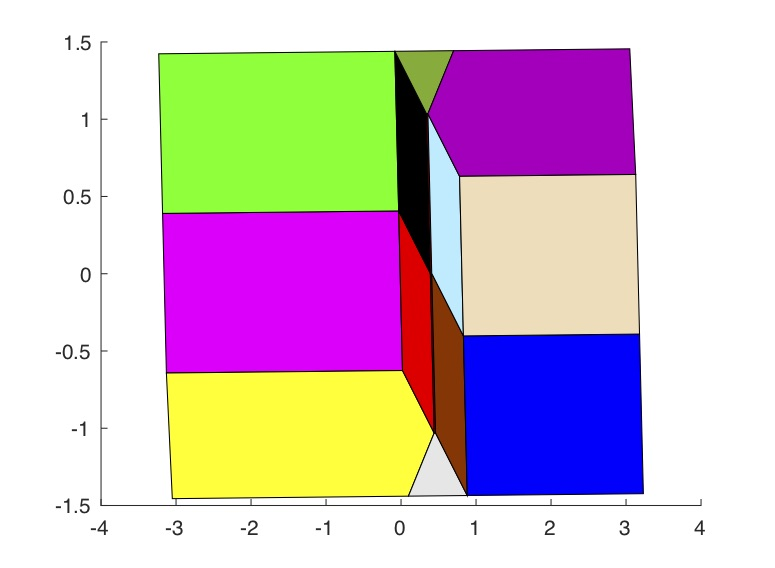
\includegraphics[width=.08\textwidth]{Figs/regs.jpg}};
			\node [block, scale=1,right=2.5cm of RMPC,
			node distance=5cm,text width=4cm] (mixed) {Finite precision implementation (computed by Daisy)};
			\node [draw, diamond, 
			minimum height=3em, minimum width=3em, right =1cm of mixed,
			node distance=5cm] (decide) {$e\leq \bar \Delta$};
			\node [block, right of=decide,
			node distance=3cm] (done) {Done};
			\node [block, below of= decide,
			node distance=3cm] (delta) {increase $\Delta$};
			\node [scale=1] at (3,-.25)  {
				$u(x)=Kx+v$
			};
		\node at (9,-.25) {$e$};
			
			
			\draw [draw,->] (RMPC) -- node [pos=-.1] {}(mixed);
			\draw [->] (mixed) -- node [name=aaa] {}(decide);
			\draw [->] (decide) -- node [above,pos=.3] {Yes} (done);
			\draw [->] (decide) -- node[pos=0.99] {} 
			node [] {No} (delta);
			\draw [->] (delta) -| node [above] {} (RMPC);
	
	\end{tikzpicture}
	\caption{high-level description of the proposed memory-efficient robust MPC design}
	\label{fig:overview}
\end{figure*}

	